\documentclass[a4paper,10pt]{article}
\setlength{\parindent}{0cm}
\usepackage{amsmath, amssymb, amsthm, mathtools,pgfplots}
\usepackage{graphicx,caption}
\usepackage{verbatim}
\usepackage{venndiagram}
\usepackage[cm]{fullpage}
\usepackage{fancyhdr}
\usepackage{tikz}
\usepackage{listings}
\usepackage{color,enumerate,framed}
\usepackage{color,hyperref}
\definecolor{darkblue}{rgb}{0.0,0.0,0.5}
\hypersetup{colorlinks,breaklinks,
            linkcolor=darkblue,urlcolor=darkblue,
            anchorcolor=darkblue,citecolor=darkblue}
\usetikzlibrary{arrows}
%\usepackage{tgadventor}
%\usepackage[nohug]{diagrams}
\usepackage[T1]{fontenc}
%\usepackage{helvet}
%\renewcommand{\familydefault}{\sfdefault}
%\usepackage{parskip}
%\usepackage{picins} %for \parpic.
%\newtheorem*{notation}{Notation}
%\newtheorem{example}{Example}[section]
%\newtheorem*{problem}{Problem}
\theoremstyle{definition}
%\newtheorem{theorem}{Theorem}
%\newtheorem*{solution}{Solution}
%\newtheorem*{definition}{Definition}
%\newtheorem{lemma}[theorem]{Lemma}
%\newtheorem{corollary}[theorem]{Corollary}
%\newtheorem{proposition}[theorem]{Proposition}
%\newtheorem*{remark}{Remark}
%\setcounter{section}{1}

\newtheorem{thm}{Theorem}[section]
\newtheorem{lemma}[thm]{Lemma}
\newtheorem{prop}[thm]{Proposition}
\newtheorem{cor}[thm]{Corollary}
\newtheorem{defn}[thm]{Definition}
\newtheorem*{examp}{Example}
\newtheorem{conj}[thm]{Conjecture}
\newtheorem{rmk}[thm]{Remark}
\newtheorem*{nte}{Note}
\newtheorem*{notat}{Notation}

%\diagramstyle[labelstyle=\scriptstyle]

\lstset{frame=tb,
  language=Oz,
  aboveskip=3mm,
  belowskip=3mm,
  showstringspaces=false,
  columns=flexible,
  basicstyle={\small\ttfamily},
  breaklines=true,
  breakatwhitespace=true,
  tabsize=3
}


\pagestyle{fancy}




\fancyhead{}
\renewcommand{\headrulewidth}{0pt}

\lfoot{\color{black!60}{\sffamily Zhangsheng Lai}}
\cfoot{\color{black!60}{\sffamily Last modified: \today}}
\rfoot{\textsc{\thepage}}



\begin{document}
\flushright{Zhangsheng Lai\\1002554}
\section*{Machine Learning: Homework 4}


\begin{enumerate}
\item For (a) and (b), as $D$ is not part of the requirement, we assume $D$ to be a variable that is not connected to any of the other variables when represented as a DAG.

\begin{enumerate}[(a)]
\item True. Consider $B$ to be that event of flipping a coin with probability of heads to be $p$, $A$ to be the event that it mirrors the outcome of the coin flip with probability 1 and $C$ to be the event that it mirrors the opposite of the outcome of the coin flip with probability 1. There is no direct dependency between $A$ and $C$, but we see that
\begin{align*}
\mathbb{P}(A=a|B=b) :=\begin{cases}
1, & a = H, b = H\\
1, & a=T, b=T\\
0, & \text{otherwise}
 \end{cases}\\
 \mathbb{P}(C=c|B=b) :=\begin{cases}
1, & c = H, b = T\\
1, & c=T, b=H\\
0, & \text{otherwise}
 \end{cases}
\end{align*}
and observe that 
\begin{align*}
\mathbb{P}(A) = \sum_{B\in \{H,T\}}\mathbb{P}(B) \mathbb{P}(A|B) &\qquad \mathbb{P}(C) = \sum_{B\in \{H,T\}}\mathbb{P}(B) \mathbb{P}(C|B) \\
\mathbb{P}(A,C) = \sum_{B\in \{H,T\}}&\mathbb{P}(B)\mathbb{P}(A|B)\mathbb{P}(C|B)
\end{align*}
Since $\mathbb{P}(A=H)\mathbb{P}(C=H) =p(1-p) $ and $\mathbb{P}(A=H,C=H) = 0$, it is shown that $A$ and $C$ are not independent, since $p \neq 0$. Alternatively, this can be explained by the common causes effect.

\item False. Let $B$ be the event that the weather is sunny, $A$ be the event of getting heads when flipping a fair coin and $C$ be the event that is True when $A$ is heads. Clearly both $A$ and $C$ is independent of $B$, however,
\begin{align*}
1 = \mathbb{P}(C=True | A=Heads) &\neq \mathbb{P}(C=True) = 0.5 \\
0 = \mathbb{P}(C=True | A=Tails) &\neq \mathbb{P}(C=True) = 0.5 
\end{align*}	
which shows that $A$ and $C$ are not independent of each other.

\begin{figure}[h]
\centering
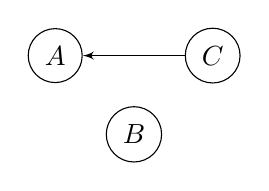
\begin{tikzpicture}

\tikzset{vertex/.style = {shape=circle,draw,minimum size=1.5em}}
\tikzset{edge/.style = {->,> = latex'}}
% vertices
\node[vertex] (a) at  (-1,1) {$A$};
\node[vertex] (c) at  (1,1) {$C$};
\node[vertex] (b) at  (0,0) {$B$};
%\node[vertex] (b) at  (0,-1.4142) {$B$};

\draw[edge] (c) to (a);
\end{tikzpicture}
\caption{Model of 1(b)}
\end{figure}


\item False. Consider the following model below,
\begin{figure}[h]
\centering
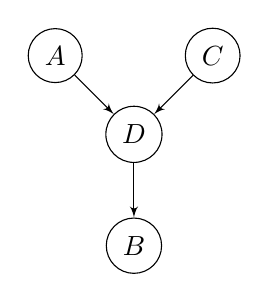
\begin{tikzpicture}

\tikzset{vertex/.style = {shape=circle,draw,minimum size=1.5em}}
\tikzset{edge/.style = {->,> = latex'}}
% vertices
\node[vertex] (a) at  (-1,1) {$A$};
\node[vertex] (c) at  (1,1) {$C$};
\node[vertex] (d) at  (0,0) {$D$};
\node[vertex] (b) at  (0,-1.4142) {$B$};

\draw[edge] (a) to (d);
\draw[edge] (c) to (d);
\draw[edge] (d) to (b);

\end{tikzpicture}
\end{figure}
we see that it fulfills the requirement that $A$ is independent of $B$ given $D$ and $C$ is independent of $B$ given $D$ by chaining. However, the explaining away effect tells us that $A$ and $C$ are dependent of each other.

\end{enumerate}
\newpage
\item
\begin{enumerate}[(a)]
\item The parameters associated with the HMM are the transmission probabilities, $a_{i,j} = p(y_{next}=j|y=i)$ for $i,j \in \{\text{START}, X,Y,Z, \text{STOP}\}$ and the emission probabilities, $b_{j}(o)=p(x=o|y=j)$ where $o \in \{a, b, c\}$ and $j \in \{X, Y, Z\}$.

\begin{table}[h]
\centering

\begin{tabular}{c|c|c|c|c}
 $a_{i,j}:$ $i \backslash j$ &$X$ & $Y$ & $Z$ & STOP\\
 \hline
 START & 1/2 &0&1/2&0\\
\hline
$X$ &2/5 & 2/5& 1/5\\
\hline
$Y$&1/5 &0 & 1/5 & 3/5 \\
\hline
$Z$ &2/5 &3/5 & 0 & 0\\
\hline
\end{tabular}
\qquad
\begin{tabular}{c|c|c|c}
$b_j(0):$$b_u(o)$ $u \backslash o$ &$a$ & $b$ & $c$\\
\hline
$X$ &2/5 & 1/5& 2/5\\
\hline
$Y$&2/5 &2/5 & 1/5 \\
\hline
$Z$ &1/5 &3/5 & 1/5\\
\hline
\end{tabular}

\end{table}

\item To solve for the probability $p(x_1=a, x_2=b)$, we use the fact that 
\begin{align}
p(y_0,\ldots, y_3,x_1,x_2) &= \prod_{i=0}^{3}a_{y_i,y_{i-1}}\prod_{i=1}^{2}b_{y_i}(x_i)\nonumber.\\ 
\text{and}~~ p(x_1=a, x_2=b) &= \sum_{\substack{y_0=\text{START},\\y_1,y_2 \in \{X,Y,Z\},\\y_3=\text{STOP}}}p(y_0,y_1,y_2, y_3,x_1=a,x_2=b) \label{eq:sum}
\end{align}
The only nonzero term in the summation of (\ref{eq:sum}) is when $y_1=Z, y_2=X$ which gives a probability of 0.00648. Thus $p(x_1=a, x_2=b)=0.00648$.
\item 
We see that $X_1, X_6$ has no parents, $X_2,X_3,X_4,X_5,X_7,X_8,X_{10},X_{11}$ has one parent each and $X_9$ has 3 parents, thus the number of free parameters is $(2 \times 1) + (8\times 2) + (1 \times 8)=26$


\item We see from the probability tables that $X_3$ is independent of $X_2$ and $X_{10}$ is independent of $X_9$. Thus $X_1$ is independent of $X_3$ and $X_{11}$ is independent of $X_9$. Thus 
\begin{align*}
P(X_5 = 2 | X_3 =1, X_{11}=2, X_1 = 1) = P(X_5=2|X_3=1)&=\sum_{v\in \{1,2\}}P(X_4=v|X_3)P(X_5|X_4)\\
&=(0.1 \times 0.5)  + (0.9\times 0.4) = 0.41
\end{align*}
\end{enumerate}

\end{enumerate}



\end{document}